\makeatletter
\def\input@path{{etc/}{body/}}
\makeatother

\documentclass[ALICE,manyauthors]{StrinJet}
\usepackage{StrinJet}

\begin{document}

\title{Multiplicity dependence of strange and multi-strange particle in jets in \pp collisions at \seven}
\author{authors}
\begin{abstract}
	\label{sec:Abs}
%1807.11321
Comprehensive results on the production of unidentified charged particles, $\pi^{\pm}$, $\mathrm{K^{\pm}}$, p, \kzero, \kstar, $\phi$, $\Lambda$, $\Xis$, $\Oms$ hadrons in jets in proton-proton (\pp) collisions at \seven  are presented
%1507.02091v2
with two developed color reconnection models, the new color reconnection model and the rope hadronization model, in PYTHIA 8 generator. The observables are ratios of identified hadron yields as a function of the transverse momentum ($\pT$) and the final-state activity (the charged multiplicity).


\end{abstract}


\setcounter{page}{1}


%\clearpage
\section{Introduction}
\label{sec:intro}
%1601.03658v2
In heavy-ion collisions at ultra-relativistic energies, it is well established that a strongly coupled Quark-Gluon-Plasma~(QGP) is formed~\cite{Adams:2005dq, Adcox:2004mh, Arsene:2004fa, Back:2004je, Schukraft:2011na}.
Recent measurements in high multiplicity \pp, p--A and d--A collisions at different energies have revealed strong flow-like effects even in these small collision systems~\cite{Abelev:2012sk, Chatrchyan:2013eya, Khachatryan:2010gv, CMS:2012qk, Abelev:2012ola, Aad:2012gla, Aad:2013fja, Chatrchyan:2013nka, Adare:2013esx, Adams:2006nd}.
%1807.11321
The baryon-to-meson ratios p/$\pi$ and $\Lambda/\kzero$, in \pp and \pPb collision systems, exhibit a characteristic depletion at $\pT \sim 0.7$~\GeVc and an enhancement at intermediate $\pT$ ($\sim$ 3~\GeVc), which is qualitatively similar to that observed in \PbPb collisions~\cite{ALICE:2018pal}.
In a letter~\cite{ALICE:2016fzo}, the ALICE Collaboration reported the multiplicity dependent enhancement of strange (\kzero, \lmb and \almb) and multi-strange (\X, \Ix, \Om and \Mo) particle in \pp collisions at \seven. As well as, those results were complemented by the measurement of $\pi^{\pm}$, $\mathrm{K}^{\pm}$, p, \pbar, \kstar and $\phi$ with ALICE~\cite{ALICE:2018pal}.
%1606.07424v2
Such behaviour cannot be reproduced by any of the MC models commonly used, suggesting that further developments are needed to obtain a complete microscopic understanding of strangeness production and indicating the presence of a phenomenon novel in high-multiplicity pp collisions.

%2105.04890
In a recent study, to provide further insight into the particle production mechanisms in high-multiplicity \pp and \pPb events,
%ALICE High light describe of V0 in jet paper
the ALICE Collaboration has studied baryon-to-meson ratios with a new method: by studying the ratios in two parts of the events separately -- inside jets and in the event portion perpendicular to a jet cone~\cite{ALICE:2021cvd}. 
%1408.2672
In contrast to the inclusive distribution, the $\pT$-differential $\lmb/\kzero$ ratio within jets in \pp and \pPb collisions does not exhibit baryon enhancement at intermediate $\pT$.
It is plausible that the baryon enhancement may therefore be attributable to the soft (low $Q^{2}$) component of the collision as discussed in~\cite{Cuautle:2014yda}.
%This results disfavors the hard-soft recombination models, while it is consistent with a picture in which the value of baryon/meson ratio has two independent mechanisms: i) the expansion of the soft particles of the underlying event within  a common velocity field (radial flow), and ii) the production of particles via hard parton-parton scatterings and the subsequent jet fragmentation.

In this work, inspired by this paper~\cite{ALICE:2021cvd}, we study the "strangeness to pion ratio increase with multiplicity" and the "baryon-to-meson ratio enhancement at intermediate $\pT$" with charged-particle jet probe by PYTHIA model. 
%1507.02091v2
In this contribution we consider two of the models: the new colour reconnection (CR) model~\cite{Christiansen:2015yqa, Sjostrand:2014zea} and the colour rope model~\cite{Biro:1984cf, Bierlich:2014xba, Flensburg:2011kk} in the PYTHIA 8 generator.
Both considered colour reconnection models are built upon the Lund model for string hadronization~\cite{Andersson:1983ia, Buckley:2011ms}.  In these models, outgoing partons are connected with string-like color fields, which fragment into hadrons when moving apart.

The paper is structured as follows: in Sec.~\ref{sec:model} will give a brief introduction about the models we used, the results compared to data are provided in Sec.~\ref{sec:com2da}, the predictions results can be find in Sec.~\ref{sec:predic}, and in the end, the paper will be summarized in Sec.~\ref{sec:sum},
%===========================================
%1906.03145
%This comprehensive set of data does allow for a detailed test of production models.


%1601.03658v2
%The origin of these phenomena is debated in~\cite{Shuryak:2013ke, Werner:2013ipa, Bozek:2013ska, Dumitru:2010iy, Schenke:2015aqa, Ma:2014pva, Ortiz:2013yxa}.
%It was also discussed that in small systems, mechanisms like color-reconnection may produce radial flow-like effects.

%1512.07227
%The role of strange hadron yields in searching for QGP was pointed out at an early stage~\cite{Rafelski:1982pu}.
%It was subsequently found that in high energy nucleus-nucleus (A--A) collisions at the Super Proton Synchrotron (SPS), the Relativistic Heavy Ion Collider (RHIC) and the Large Hadron Collider (LHC) the abundances of strange and multi-strange baryons are compatible with those from thermal statistical model calculations~\cite{Andersen:1998vu, NA49:2002fxd, NA57:2004nxc, NA49:2003bok, STAR:2003jis, STAR:2006egk, STAR:2007cqw, ALICE:2013xmt }

%1204.0282v3
%The multi-strange baryons, $\Omega$~(sss) and $\Xi$~(dss), are particularly important in high energy particle and nuclear physics due to their dominant strange quark~(s-quark) content. The initial state colliding projectiles contain no strange valence quark, therefore all particles with non-zero strangeness quantum number are created in the course of the collision.


%1901.07447
%The theoretical picture of collective effects in heavy ion collisions is vastly different from the picture known from \pp collisions. Due to the very different geometry of the two system types, interactions in the final state of the collision become dominant in heavy ion collisions, while nearly absent in \pp collisions.

%1612.05132
%1612.05132
%The rope model provides corrections to the string hadronization model, by allowing strings overlapping in transverse space to act coherently as a "rope". %\footnote{A Lund string is in its simplest form, a straight piece stretched between a quark and an anti-quark, or a color triplet and anti-triplet. As gluons are added to the string, they act as point-like "kinks" on the string, carrying energy and momentum~\cite{Andersson:1979ij}. We will denote all straight pieces between gluons or (anti)quarks string segments. A $q - g - \overline{q}$ string thus has two segments.}.
%To provide a description of the hadrochemistry in the underlying event of \pp collisions, it has been suggested a "rope hadronization" model~\cite{Bierlich:2014xba}, based on work by Biro, Knoll and Nielsen~\cite{Biro:1984cf}. This model provides corrections to the string hadronization model, by allowing strings overlapping in transverse space to act coherently as a "rope". The model is implemented in the DIPSY event generator~\cite{Flensburg:2011kk}, which provides a dynamical picture of the event structure in impact parameter space, allowing for a calculation of the color field strength in each small rope segment\footnote{A Lund string is in its simplest form, a straight piece stretched between a quark and an anti-quark, or a color triplet and anti-triplet. As gluons are added to the string, they act as point-lik "kinks" on the string, carrying energy and momentum~\cite{Andersson:1979ij}. We will denote all straight pieces between gluons or (anti)quarks string segments. A $q - g - \overline{q}$ string thus has two segments.}. This formalism also includes all fluctuations. The color field is characterized by two quantum numbers ${p, q}$, which together signifies its SU(3) multiplet structure. Lattice calculations have shown~\cite{Bali:2000un}, that the string tension -- energy per unit length -- scales with the quadratic Casimir operator of the multiplet, such that the ratio of the enhanced rope tension ($\widetilde{\kappa}$) to the triplet string tension in vacuum $\kappa$ is:



\section{Models}
\label{sec:model}
%describe the models we used (Rope and CR)
\subsection{New color reconnection model}
\label{subsec:cr}

\subsection{Color rope model}
\label{subsec:rope}

%1412.6259v3
As rope formation is expected to give increased rates of strange particles and baryons, which may mimic effects of plasma formation, it makes signals for a phase transition more difficult to interpret.
It has also been suggested that ropes may initiate the formation of a quark–gluon plasma~\cite{Gyulassy:1985oqt, Kajantie:1985jh, Gatoff:1987uf, Braun:1997ch}.
At LHC energies many overlapping strings are also expected in \pp scattering, where plasma formation normally is not expected.

\section{Compare to data}
\label{sec:com2da}
%1507.02091v2
The models performs as intended when comparing to existing data.
%1806.11390
The inclusive measurements on the charged particle pseudo-rapidity and multiplicity distributions are presented in Figure~\ref{fig:trkinfo}.
\begin{figure}[htp]
	\begin{center}
		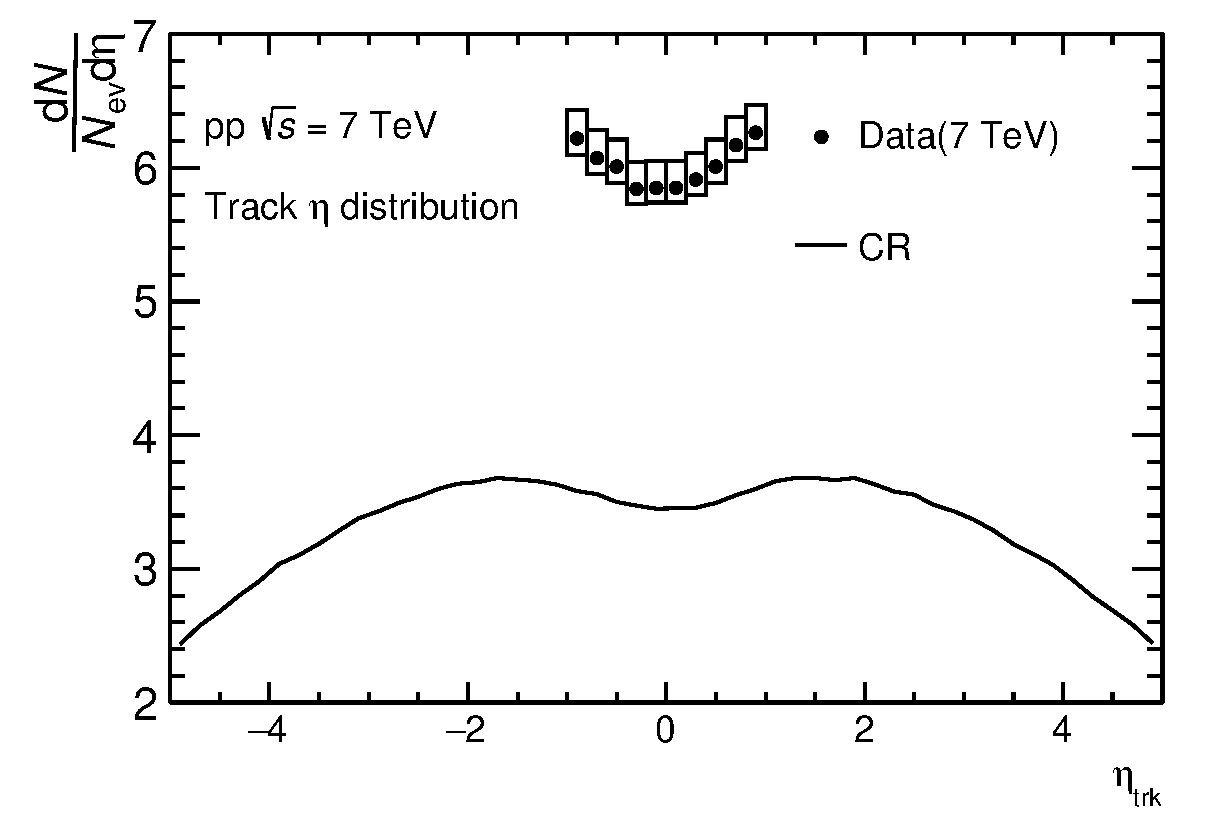
\includegraphics[width=.49\textwidth]{TrkEta}
		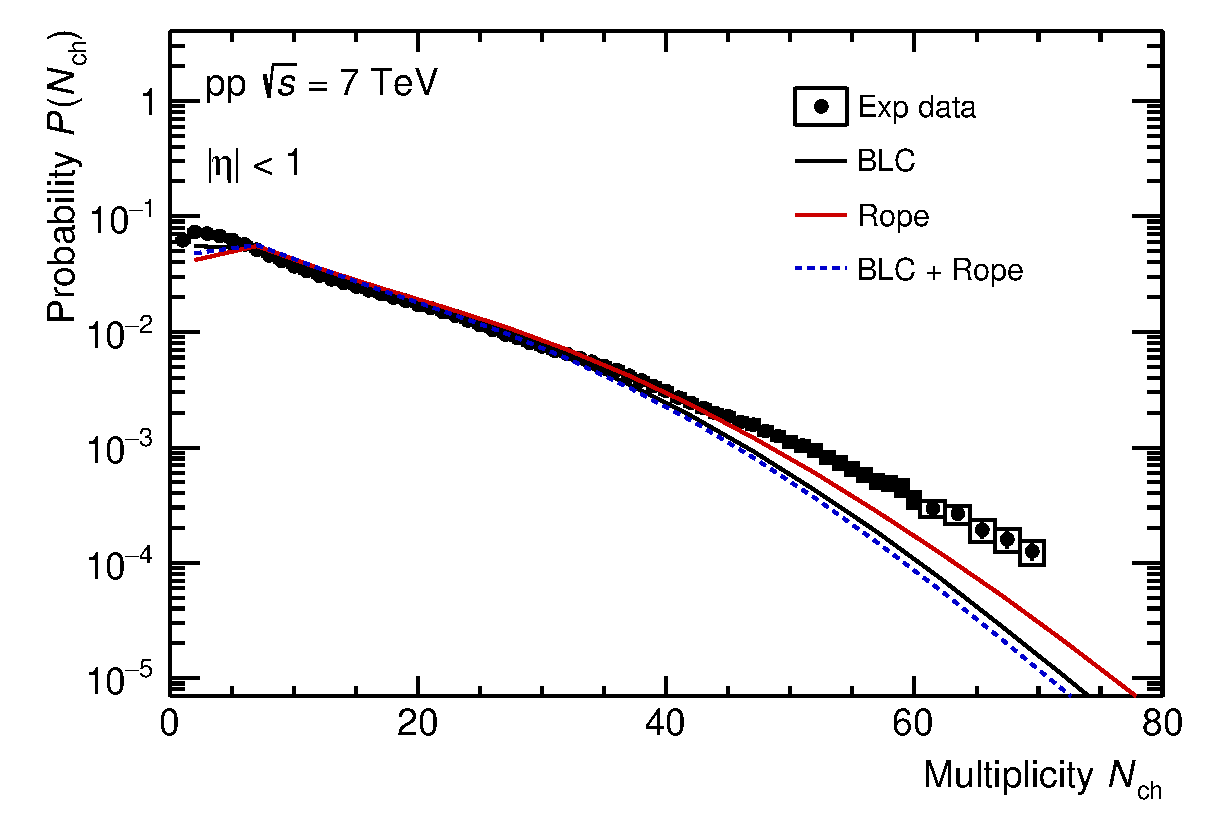
\includegraphics[width=.49\textwidth]{dNmiddEta}
	\end{center}
	\caption{Charged particle pseudo-rapidity ($\eta_\mathrm{trk}$)(left) and number of mid-rapidity tracks ($N_\mathrm{mid}$) (right) distribution for \pp collisions at \seven.  The experimental data are taken from~\cite{ALICE:2010mty}.}
	\label{fig:trkinfo}
\end{figure}


\section{Predictions}
\label{sec:predic}

\section{Summary}
\label{sec:sum}


\newenvironment{acknowledgement}{\relax}{\relax}
%\begin{acknowledgement}
%\section*{Acknowledgements}
%\input{acknowledgements.tex}

%\end{acknowledgement}

\bibliographystyle{etc/utphys}
\bibliography{StrinJet}

\newpage
\appendix
\section{Model parameters}
\label{app:modpara}

\begin{table}[ht]
\label{tab:CRparameter}
  \begin{center}
  \begin{tabular}{|c|c|}
	\hline
	  Parameters & Values \\
	\hline 
	MultiPartonInteractions:pT0Ref &  2.15\\ 
	BeamRemnants:remnantMode & 1 \\
	BeamRemnants:saturation & 5 \\
	ColourReconnection:reconnect & on \\
	ColourReconnection:mode & 1 \\
	ColourReconnection:allowDoubleJunRem & off \\
	ColourReconnection:m0 & 0.3  \\
	ColourReconnection:allowJunctions & on \\
	ColourReconnection:junctionCorrection & 1.2 \\;
	ColourReconnection:timeDilationMode & 2 \\
	ColourReconnection:timeDilationPar & 0.18\\ 
	\hline 
  \end{tabular} 
  \caption{Colour reconnection model parameters}
  \end{center}
\end{table}

\begin{table}[ht]
	\label{tab:Ropeparameter}
	\begin{center}
		\begin{tabular}{|c|c|}
			\hline
			Parameters & Values \\
			\hline 
			Ropewalk:RopeHadronization & on \\
			Ropewalk:doShoving & on  \\
			Ropewalk:tInit & 1.5 \\
			Ropewalk:deltat & 0.05 \\
			Ropewalk:tShove & 0.1 \\
			Ropewalk:gAmplitude & 0. \\
			Ropewalk:doFlavour & on \\
			Ropewalk:r0 & 0.5 \\
			Ropewalk:m0 & 0.2 \\
			Ropewalk:beta & 0.1 \\
			\hline 
		\end{tabular} 
		\caption{Rope hadronization model parameters}
	\end{center}
\end{table}
%\input{} % put your appendices here (if any)
 
\end{document}
